\documentclass[prd,aps,preprint,superscriptaddress,nofootinbib,amsmath,amssymb,eqsecnum]{revtex4-2}

\usepackage[T1]{fontenc}
\usepackage[utf8]{inputenc}
\usepackage{booktabs,array}
\usepackage{xcolor}
\usepackage{tikz}
\usetikzlibrary{arrows.meta,positioning,shapes.geometric}
\usepackage[colorlinks=true,allcolors=blue]{hyperref}

% ---- notation ---------------------------------------------------------
\newcommand{\W}{\mathcal{W}}
\newcommand{\pmeas}[2][d]{\frac{d^{#1}#2}{(2\pi)^{#1}}\,}
\newcommand{\tomega}{\tilde{\omega}}
\newcommand{\p}{\tilde{\phi}}
\newcommand{\G}{\tilde{G}}
\newcommand{\todo}[1]{\textcolor{red}{[#1]}}
\newcommand{\ip}[1]{\int_{#1}}

% author-note symbols: start at dagger instead of asterisk
\makeatletter
\def\@fnsymbol#1{\ensuremath{\ifcase#1\or \dagger\or \ddagger\or \mathsection\or
  \mathparagraph\or \|\or \dagger\dagger\or \ddagger\ddagger\else\@ctrerr\fi}}
\makeatother

\begin{document}

\title{Reconstructing the Goldberg--Palatini Action from Noether Identities}

\author{F. T. Brandt}
\email{fbrandt@usp.br}
\affiliation{Instituto de F\'{\i}sica, Universidade de S\~ao Paulo, S\~ao Paulo, SP 05508-090, Brazil}
\author{Augusto C. B. Carvalho}
\email{augusto.burlacchini@usp.br}
\affiliation{Instituto de F\'{\i}sica, Universidade de S\~ao Paulo, S\~ao Paulo, SP 05508-090, Brazil}

\date{\today}

\begin{abstract}
We investigate the reconstruction of the first-order gravitational action from the Noether
identities associated with diffeomorphism invariance. The independent fields are a symmetric
perturbation of the contravariant metric density and an independent trace-adjusted
connection, with prescribed transformation laws. In generic spacetime dimension, we construct a local,
Lorentz-covariant ansatz containing quadratic terms with at most two derivatives and a cubic
interaction restricted to the structure $\phi GG$. The action kernels are expanded in tensor
bases comprising 31 independent coefficients. Expanding the Noether identities order by order
in the fields yields algebraic constraints, which we solve using symbolic computation. These
constraints eliminate the $\phi\phi$ kernel and determine the remaining coefficients up to an
overall normalization, recovering the Goldberg--Palatini action. Since the connection can be
eliminated exactly, the result also determines the complete
second-order action, with its infinite set of graviton vertices. The construction requires no
choice of an energy--momentum tensor to guide the self-coupling procedure and directly
identifies the restrictions imposed by the prescribed symmetry. The result establishes
uniqueness within the assumed class of actions. All tensor bases, identities and solutions are
provided in appendices, and the symbolic computations will be made available as
supplementary material.
\end{abstract}

\maketitle


% =======================================================================
\section{Introduction}
\label{sec:introduction}
% =======================================================================

The extent to which gravitational dynamics can be recovered from the consistency of an
interacting massless spin-two field is a longstanding question. In the self-coupling
construction, which goes back to Feynman~\cite{Feynman1995} and was completed by
Deser~\cite{Deser1970}, the use of first-order variables allows the nonlinear completion to
be expressed through a cubic interaction, avoiding the infinite expansion of the metric
formulation. Discussions of this approach have also emphasized the
assumptions entering the construction, the ambiguities in the energy--momentum tensor, and the
treatment of boundary terms~\cite{Padmanabhan2008,Deser2010}. These issues motivate a
formulation in which the constraints imposed by gauge symmetry can be examined directly.

Local gauge invariance implies differential identities among the Euler--Lagrange derivatives
of the action. These are identities of Noether's second theorem and hold off shell. Once the
field transformations and a class of admissible actions have been specified, they can be used
as algebraic conditions on unknown interaction coefficients. This reverses the usual direction
of the calculation: instead of deriving identities from a known action, one uses the
identities to determine which actions are compatible with the prescribed transformations.
This strategy was used in Ref.~\cite{BrandtElias2006} to determine the scalar--graviton
vertex in noncommutative space, where the closed form of the action is not available, from
the invariance under a restricted class of coordinate transformations.

In this work we apply this strategy to the first-order gravitational variables $\phi^{\mu\nu}$
and $G^{\lambda}{}_{\mu\nu}$. The former is the perturbation of the contravariant metric
density, while the latter is a trace-adjusted connection treated as an independent field. The
same strategy applies in the metric formulation, where the field-dependent part of the
transformation is essential: invariance under the linearized transformations alone fixes
only part of each vertex, whereas the full transformation determines the three-graviton
vertex from the quadratic term, up to total derivatives~\cite{BrandtFrenkel1996}. The
programme does not terminate there, however, since new vertices appear at every order. The first-order choice is adapted to the polynomial
structure of the Goldberg--Palatini action~\cite{Goldberg1958,Palatini1919,Ferraris1982} and
to its use in perturbative gravity~\cite{BrandtMcKeon2016}. We restrict the action to quadratic kernels of
prescribed derivative order and to a derivative-free cubic interaction of the form $\phi GG$,
expand the kernels in tensor bases, and impose the Noether identities order by order in the
fields; the determination of the action then reduces to a finite system of linear constraints on 31
coefficients, which is solved completely.

The result is not confined to the first-order theory. The field equation of $G$ is
algebraic, so once the first-order action is fixed the connection can be eliminated
exactly, for $d>2$ and nondegenerate metric density: $G$ is expressed through
$\partial\phi$ by inverting the kernel of the $GG$ term, which is linear in
$\eta+\kappa\phi$, and substituting back gives the second-order action as a quadratic form
in $\partial\phi$ whose kernel is that inverse, Eq.~(3.13) of Ref.~\cite{BrandtMcKeon2016}.
The formal perturbative expansion of the inverse, Eq.~(3.18) there,
then generates the complete infinite set of graviton self-interaction vertices of the metric
formulation. The finite determination of the first-order action therefore fixes all of them.

Our objective is to determine the freedom remaining in this ansatz after the Noether
identities are imposed. The transformation laws, the field content, the derivative bounds and
the restriction on the cubic interaction are inputs to the construction. Accordingly, the
uniqueness statement concerns this specified class of actions; it does not assert that
diffeomorphism invariance alone selects Einstein gravity among all local gravitational
theories.

The present construction complements the self-coupling approach of
Refs.~\cite{Deser1970,Deser2010} by determining the admissible action kernels directly from
prescribed nonlinear gauge transformations. Its contribution is an explicit finite-dimensional
uniqueness analysis within the stated ansatz, identifying which Noether identities remove
each remaining freedom. The self-coupling procedure has
recently been extended to metric-affine theories, with the connection as an independent
field~\cite{Delhom2023}; that analysis identifies the choice of energy--momentum tensor as
the source of the ambiguities, notes that in the first-order construction of
Ref.~\cite{Deser1970} the connection is an auxiliary field that is not itself bootstrapped,
and observes that the existing arguments establish existence rather than uniqueness. The
present construction, within the stated ansatz, addresses these three points: no
energy--momentum tensor is chosen, which is the point at issue in
Ref.~\cite{Padmanabhan2008}, the geometrical input being retained explicitly in the
transformation laws; the variations of both independent fields enter the Noether identity
and are included in the determination; and uniqueness is established within the stated
class. The idea of using the consistency of the gauge identities instead of self-coupling
goes back to Wald~\cite{Wald1986}, who analyzed the consistent nonlinear extensions through
identities among the field equations; here the nonlinear transformations are prescribed and
the compatible action is determined within a finite ansatz. The result concerns the bulk action modulo total derivatives and
does not determine boundary terms.

The distinction can also be expressed in terms of Noether's two theorems. Energy--momentum
self-coupling constructions combine the conserved current associated with global translations
with the consistency conditions imposed by the gauge identities of the spin-two field. Here
we impose the off-shell identities of Noether's second theorem directly, without constructing
an energy--momentum tensor as an intermediate step. Translation symmetry is already contained
in the prescribed transformations. The difference therefore lies in the organization and
inputs of the procedure: the nonlinear transformations are specified at the outset,
and the compatible action is determined within the chosen ansatz.

The paper is organized so that the main text carries the logic of the construction and the
appendices carry its details. Section~\ref{sec:variables} fixes the fields and their
transformations, Section~\ref{sec:ansatz} the ansatz and its counting, Section~\ref{sec:identities}
the identities and their decomposition into sectors, Section~\ref{sec:solution} the solution,
and Section~\ref{sec:checks} the checks and the scope of the result. Figure~\ref{fig:flow}
summarizes the procedure. Explicit tensors, bases, identities and kernels are collected in
Appendices~\ref{app:momentum}--\ref{app:kernels}, and Appendix~\ref{app:implementation}
describes the symbolic implementation and how to reproduce every check.

% =======================================================================
\section{First-order variables and gauge transformations}
\label{sec:variables}
% =======================================================================

\paragraph{Conventions.} Units are $\hbar=c=1$, so that dimensions are mass dimensions. We
work in $d$ spacetime dimensions with a flat metric $\eta_{\mu\nu}$ of signature
$(+,-,\dots,-)$; the algebraic tensor identities used below are polynomial identities in
$\eta$ and the momenta and are independent of the signature, and for generic $d$ the density
$\sqrt{-g}$ is to be read as $\sqrt{|g|}$. Index symmetrization is \emph{not} normalized:
$h^{(\mu\nu)}\equiv h^{\mu\nu}+h^{\nu\mu}$. Fourier transforms are
$\p^{\mu\nu}(p)=\int d^dx\,e^{ip\cdot x}\phi^{\mu\nu}(x)$, and likewise for
$\G^{\lambda}{}_{\mu\nu}$ and for the gauge parameter $\tomega^\mu$, so that
$\phi^{\mu\nu}(x)=\ip{p}e^{-ip\cdot x}\p^{\mu\nu}(p)$ with $\ip{p}\equiv\int d^dp/(2\pi)^d$;
a derivative acting on a field of momentum $p$ becomes $-ip_\mu$, and a product of fields
becomes a convolution. Table~\ref{tab:notation} lists the objects used throughout.

\paragraph{Compact notation.} In the main text we suppress indices. A field carries its
momentum as a subscript: $\phi_p$ stands for the whole tensor
$\p^{\mu\nu}(p)$, $G_p$ for $\G^{\lambda}{}_{\mu\nu}(p)$, $\omega_p$ for $\tomega^\mu(p)$;
the index structure of each is that of Table~\ref{tab:notation}. The objects that act on
fields are of three kinds.
\begin{itemize}
\item A \emph{kernel} $K$ is a multilinear form on fields: $K(A,B)$ or $K(A,B,C)$ denotes the
full contraction of the indices of each argument with the corresponding index group of the kernel $K$.
For instance,
$K^{\phi G}(\phi_{-p},G_p)\equiv\p^{\mu\nu}(-p)\,K^{\phi G}_{\mu\nu\lambda}{}^{\rho\sigma}(p)\,\G^{\lambda}{}_{\rho\sigma}(p)$.
\item A \emph{linear map} $D(p)$ takes the gauge parameter to a field:
$D_{\phi^0}(p)\,\omega_p\equiv D_{\phi^0}{}^{\mu\nu}{}_{\alpha}(p)\,\tomega^\alpha(p)$ is a
symmetric tensor, and likewise $D_{G^0}(p)\,\omega_p$. The label of a $D$ names the field it
produces and the order in $\kappa$ of the term of the transformation from which it arises:
$D_{\phi^0}$ is the field-independent part of $\delta\phi$, $D_{\phi^1}$ the part linear in
the fields, Eq.~\eqref{eq:dmom} below.
\item A \emph{bilinear map} $D(p,q)$ takes a field and the gauge parameter to a field,
\[
D_{\phi^1}(p,q)(\phi_{p-q},\omega_q)\equiv\p^{\alpha\beta}(p-q)\,\tomega^\rho(q)\,
D_{\phi^1}{}^{\mu\nu}{}_{\alpha\beta\rho}(p,q),
\]
and likewise $D_{G^1}(p,q)(G_{p-q},\omega_q)$.
\end{itemize}
The index structure of every object is given in Table~\ref{tab:kernels} and in the
appendices; the compact form is only a shorthand for those expressions.

\begin{table}[htb]
\centering\scriptsize
\begin{tabular}{@{}lllcc@{}}
\toprule
Symbol & Meaning & Indices & Momenta & Dimension \\
\midrule
$\kappa$ & gravitational coupling & & & $(2-d)/2$ \\
$\phi^{\mu\nu}$; $\phi_p$ & density perturbation, Eq.~\eqref{eq:Gdef} & $\mu\nu$ symmetric & one & $(d-2)/2$; $-(d+2)/2$ \\
$G^{\lambda}{}_{\mu\nu}$; $G_p$ & trace-adjusted connection, Eq.~\eqref{eq:Gdef} & $\mu\nu$ symmetric & one & $d/2$; $-d/2$ \\
$\omega^{\mu}$; $\omega_p$ & gauge parameter & vector & one & $(d-4)/2$; $-(d+4)/2$ \\
$D_{\phi^0}(p)$, $D_{G^0}(p)$ & $\delta^{(0)}\phi$, $\delta^{(0)}G$ as maps on $\omega$ & App.~\ref{app:momentum} & $p$ & $1$, $2$ \\
$D_{\phi^1}(p,q)$, $D_{G^1}(p,q)$ & $\delta^{(1)}\phi$, $\delta^{(1)}G$ as maps on (field,\,$\omega$) & App.~\ref{app:momentum} & $p,q$ & $1$, $1$ \\
$K^{\phi\phi}$, $K^{\phi G}$, $K^{GG}$ & quadratic kernels of $S_2$ & Table~\ref{tab:kernels} & $p$ & $2$, $1$, $0$ \\
$K^{\phi GG}$ & cubic kernel of $S_3$ & Table~\ref{tab:kernels} & none & $0$ \\
$\W^{\phi},\W^{G},\W^{31},\dots,\W^{34}$ & the six Noether identities & App.~\ref{app:identities} & $p$; $p_i$ & \\
\bottomrule
\end{tabular}
\caption{Notation and mass dimensions. For the fields and the gauge parameter the two entries
in the last column refer to configuration and momentum space; $[\ip{p}]=d$.}
\label{tab:notation}
\end{table}

\paragraph{Fields.} The independent fields are the perturbation of the Goldberg
density~\cite{Goldberg1958} and
the trace-adjusted connection, both normalized with the gravitational coupling $\kappa$,
\begin{equation}
\kappa\,\phi^{\mu\nu}=\sqrt{-g}\,g^{\mu\nu}-\eta^{\mu\nu},\qquad
\kappa\,G^{\lambda}{}_{\mu\nu}=\Gamma^{\lambda}{}_{\mu\nu}
-\tfrac12\big(\delta^{\lambda}_{\mu}\Gamma^{\sigma}{}_{\nu\sigma}
+\delta^{\lambda}_{\nu}\Gamma^{\sigma}{}_{\mu\sigma}\big),
\label{eq:Gdef}
\end{equation}
both real and symmetric in $\mu\nu$. Here $\Gamma^{\lambda}{}_{\mu\nu}$ is an independent
symmetric affine connection, the Palatini variable~\cite{Palatini1919,Ferraris1982}, and not
the Levi-Civita connection built
from $g_{\mu\nu}$: for the action found below, the field equation of $\Gamma$ identifies the
two when $d>2$ and the metric is nondegenerate, and that equation is not imposed in the
construction. The second relation in Eq.~\eqref{eq:Gdef} is a linear change of variables,
invertible for $d\neq1$. Taking its trace
gives $\Gamma^{\sigma}{}_{\nu\sigma}=\frac{2\kappa}{1-d}\,g_\nu$, with
$g_\nu\equiv G^{\sigma}{}_{\nu\sigma}$, and substituting back,
\begin{equation}
\Gamma^{\lambda}{}_{\mu\nu}=\kappa\Big[G^{\lambda}{}_{\mu\nu}
+\frac{1}{1-d}\big(\delta^{\lambda}_{\mu}\,g_\nu+\delta^{\lambda}_{\nu}\,g_\mu\big)\Big],
\label{eq:GammaofG}
\end{equation}
Eqs.~(6)--(8) of Ref.~\cite{BrandtMcKeon2015}. The trace adjustment is what cancels the
$\partial_\nu\Gamma^{\lambda}{}_{\mu\lambda}$ term of $h^{\mu\nu}R_{\mu\nu}(\Gamma)$ against
the trace part of $\partial_\lambda\Gamma^{\lambda}{}_{\mu\nu}$, leaving the single derivative
term of Eq.~\eqref{eq:result} below. With
$[\kappa]=(2-d)/2$ in mass units, $\kappa\phi$ is dimensionless, $[\phi]=(d-2)/2$, and
$[G]=d/2$; in $d=4$, $[\phi]=1$ and $[G]=2$. Note that $G$ does not have the dimension of a
connection: it is the trace-adjusted connection divided by $\kappa$, in the same way that
$\phi$ is the metric perturbation divided by $\kappa$. The definitions in
Eqs.~\eqref{eq:Gdef}--\eqref{eq:GammaofG} serve only to fix the transformation laws below;
from then on $\phi$ and $G$ are treated as independent fields, and no relation between $G$ and
a metric is assumed.

\paragraph{Transformations.} Under an infinitesimal diffeomorphism
$x^\mu\to x^\mu-\kappa\,\omega^\mu(x)$ the fields transform as
\begin{align}
\delta\phi^{\mu\nu}&=
\underbrace{\eta^{\mu\nu}\partial\!\cdot\!\omega-\partial^{(\mu}\omega^{\nu)}}_{\delta^{(0)}\phi^{\mu\nu}}
+\kappa\,\underbrace{\big[\partial_\rho(\phi^{\mu\nu}\omega^\rho)-\partial_\rho\omega^{(\mu}\phi^{\nu)\rho}\big]}_{\delta^{(1)}\phi^{\mu\nu}},
\label{eq:dphi}\\
\delta G^{\lambda}{}_{\mu\nu}&=
\underbrace{\partial_\mu\partial_\nu\omega^\lambda-\tfrac12\delta^{\lambda}_{(\mu}\partial_{\nu)}\partial\!\cdot\!\omega}_{\delta^{(0)}G^{\lambda}{}_{\mu\nu}}
+\kappa\,\underbrace{\big[\omega^\rho\partial_\rho G^{\lambda}{}_{\mu\nu}-G^{\rho}{}_{\mu\nu}\partial_\rho\omega^\lambda
+G^{\lambda}{}_{\rho(\mu}\partial_{\nu)}\omega^\rho\big]}_{\delta^{(1)}G^{\lambda}{}_{\mu\nu}}.
\label{eq:dG}
\end{align}
The gauge parameter has $[\omega]=(d-4)/2$, so that it is dimensionless in $d=4$. The
split into a field-independent contribution $\delta^{(0)}$ and a field-linear contribution
$\kappa\delta^{(1)}$, of order $\kappa$, is what organizes the whole construction.
Eq.~\eqref{eq:dphi} follows from the transformation of $h^{\mu\nu}=\eta^{\mu\nu}+\kappa\phi^{\mu\nu}$
as a tensor density of weight one, with the background $\eta^{\mu\nu}$ held fixed;
Eq.~\eqref{eq:dG} follows from the transformation of an affine connection through
Eq.~\eqref{eq:Gdef}. Both are derived in Appendix~\ref{app:transf}; they are
Eqs.~(17b) and (18) of Ref.~\cite{BrandtMcKeon2015}. These two laws are the only input of the
construction beyond the class of actions defined in the next section.

In momentum space the derivatives become momenta and $\delta^{(1)}$ becomes a convolution:
\begin{equation}
\delta\phi_p=D_{\phi^0}(p)\,\omega_p+\kappa\ip{q}D_{\phi^1}(p,q)\,(\phi_{p-q},\omega_q),\qquad
\delta G_p=D_{G^0}(p)\,\omega_p+\kappa\ip{q}D_{G^1}(p,q)\,(G_{p-q},\omega_q).
\label{eq:dmom}
\end{equation}
This form makes the structure explicit: $\delta^{(0)}$ is a linear map on the gauge parameter,
$\delta^{(1)}$ a bilinear map on the pair (field, gauge parameter). The four tensors
$D_{\phi^0},D_{\phi^1},D_{G^0},D_{G^1}$ are listed in Appendix~\ref{app:momentum}.

% =======================================================================
\section{The action ansatz}
\label{sec:ansatz}
% =======================================================================

We look for an action $S=S_2+\kappa S_3$, quadratic plus cubic in the fields, of the form
\begin{equation}
\begin{aligned}
S_2&=\ip{p}\Big[K^{\phi\phi}(\phi_{-p},\phi_p)+K^{\phi G}(\phi_{-p},G_p)+K^{GG}(G_{-p},G_p)\Big],\\
S_3&=\ip{p}\ip{q}K^{\phi GG}(\phi_{p+q},G_{-p},G_{-q}).
\end{aligned}
\label{eq:ansatz}
\end{equation}
The kernels $K^{\phi\phi}$ and $K^{\phi G}$ depend on the momentum $p$; $K^{GG}$ and
$K^{\phi GG}$ do not, for the reason given below.
The quadratic part is the most general translation-invariant local expression within the
coupling-power assignment and the parity-even tensor class specified below. The cubic part
is restricted to the single structure $\phi GG$; this is an assumption, discussed below.

\paragraph{Derivative counting.} The dimensions of the fields are fixed by the
transformation laws: $\kappa\omega$ is a coordinate displacement, so $[\kappa\omega]=-1$,
and Eqs.~\eqref{eq:dphi}--\eqref{eq:dG} then give $[\phi]=(d-2)/2$ and $[G]=d/2$, consistent
with Eq.~\eqref{eq:Gdef} (see Table~\ref{tab:notation}). With these assignments $S$ carries no
prefactor, and the ansatz prescribes the power of the coupling at each order in the fields,
$\kappa^{n-2}$ in $S_n$. A local monomial with $a$ fields $\phi$, $b$ fields $G$ and $r$
derivatives, multiplied by $\kappa^{a+b-2}$, then has mass dimension $d+r+b-2$, so that a
dimensionless action requires $r+b=2$. This gives two derivatives for $K^{\phi\phi}$, one for $K^{\phi G}$ and none for $K^{GG}$;
at cubic order it allows $\phi\phi\phi$ with two derivatives, $\phi\phi G$ with one and
$\phi GG$ with none, and excludes $GGG$, which would require $r=-1$. The derivative bounds
thus rest on locality, dimensional consistency and the coupling-power assignment; they do
not by themselves bound the number of fields $\phi$. The cubic vertex $K^{\phi GG}$ is purely
algebraic, which is the feature of the first-order formulation that makes the determination
finite.

\paragraph{The cubic sector.} The restriction of $S_3$ to the structure $\phi GG$ is an
assumption: the counting above also allows $\phi\phi G$ with one derivative and
$\phi\phi\phi$ with two, and both would keep the field equation of $G$ algebraic. The
restriction is motivated by the polynomial structure of the Goldberg--Palatini action, in
which the connection appears at most quadratically and the only derivative acts in the
$\phi G$ term; it defines the class in which we investigate whether the Noether identities
admit a completion terminating at cubic order. The uniqueness result of
Section~\ref{sec:solution} is conditional on this restriction, and its relaxation is
discussed in Section~\ref{sec:conclusions}.

\paragraph{Tensor bases.} Each kernel is expanded in a basis of tensors built from
$\eta^{\mu\nu}$ and $p^\mu$, with the index symmetries inherited from the fields it
multiplies; parity-odd structures involving the Levi-Civita tensor are not considered. The bases are generated by symmetrizing, under the index symmetries of each
kernel, the tensor monomials, that is, the products of $\eta$'s and $p$'s with the required
indices and degree in $p$; their linear independence is verified through Gram determinants
(Appendix~\ref{app:bases}). Table~\ref{tab:kernels} gives the outcome. For $d\geq4$ the
four bases are independent and contain $4+6+5+16=31$ unknown coefficients in total.

\begin{table}[htb]
\centering
\begin{tabular}{@{}lllcc@{}}
\toprule
Kernel & Index symmetries & Momentum & Monomials & Basis dimension \\
\midrule
$K^{\phi\phi}_{\mu\nu\rho\sigma}$ & $\mu\leftrightarrow\nu$, $\rho\leftrightarrow\sigma$, $(\mu\nu)\leftrightarrow(\rho\sigma)$ & $p^2$ & $p^2\eta\eta$, $pp\eta$ & 4 \\
$K^{\phi G}_{\mu\nu\lambda\rho\sigma}$ & $\mu\leftrightarrow\nu$, $\rho\leftrightarrow\sigma$ & $p$ & $p\eta\eta$ & 6 \\
$K^{GG}_{\lambda\mu\nu\rho\sigma\tau}$ & $\mu\leftrightarrow\nu$, $\sigma\leftrightarrow\tau$, $(\lambda\mu\nu)\leftrightarrow(\rho\sigma\tau)$ & $p^0$ & $\eta\eta\eta$ & 5 \\
$K^{\phi GG}_{\mu\nu\lambda\alpha\beta\rho\sigma\tau}$ & $\mu\leftrightarrow\nu$, $\alpha\leftrightarrow\beta$, $\sigma\leftrightarrow\tau$, $(\lambda\alpha\beta)\leftrightarrow(\rho\sigma\tau)$ & $p^0$ & $\eta\eta\eta\eta$ & 16 \\
\bottomrule
\end{tabular}
\caption{The four kernels of the ansatz \eqref{eq:ansatz}, their symmetries, and the
dimension of the tensor basis in which each is expanded, for $d\geq4$.}
\label{tab:kernels}
\end{table}

% =======================================================================
\section{Noether identities and their decomposition}
\label{sec:identities}
% =======================================================================

Invariance of $S$ under Eqs.~\eqref{eq:dphi}--\eqref{eq:dG}, ordered by powers of
$\kappa$, or equivalently by the number of fields, gives three identities,
\begin{equation}
\delta^{(0)}S_2=0,\qquad
\delta^{(0)}S_3+\delta^{(1)}S_2=0,\qquad
\delta^{(1)}S_3=0,
\label{eq:noether}
\end{equation}
where $\delta^{(m)}S_n\equiv\int(\delta S_n/\delta A)\,\delta^{(m)}A$ summed over the
fields $A=\phi,G$. Each identity holds for arbitrary $\omega$ and arbitrary field
configurations, so it can be decomposed further according to which fields appear. Taking
functional derivatives with respect to the fields and setting the fields to zero turns each
piece into an algebraic tensor identity among the kernels, in momentum space. The
decomposition is summarized in Table~\ref{tab:identities}; the six identities are written out
in Appendix~\ref{app:identities}. The resulting relations among the action kernels are also
called classical Ward identities, the terminology used in the accompanying notebooks; we
keep ``Noether identities'' to emphasize their derivation from Noether's second theorem.
They concern the classical action before gauge fixing, not the Green functions or the BRST
identities of a gauge-fixed theory.

\begin{table}[htb]
\centering
\begin{tabular}{@{}llllc@{}}
\toprule
Identity & From & Field sector & Kernels involved & Projection basis \\
\midrule
$\W^{\phi}$  & $\delta^{(0)}S_2$ & $\phi$   & $K^{\phi\phi}$, $K^{\phi G}$ & 3 \\
$\W^{G}$     & $\delta^{(0)}S_2$ & $G$      & $K^{\phi G}$, $K^{GG}$ & 6 \\
$\W^{31}$    & $\delta^{(1)}S_2$ & $\phi\phi$ & $K^{\phi\phi}$ & 7 \\
$\W^{32}$    & $\delta^{(0)}S_3+\delta^{(1)}S_2$ & $\phi G$ & $K^{\phi GG}$, $K^{\phi G}$ & 23 \\
$\W^{33}$    & $\delta^{(0)}S_3+\delta^{(1)}S_2$ & $GG$ & $K^{\phi GG}$, $K^{GG}$ & 20 \\
$\W^{34}$    & $\delta^{(1)}S_3$ & $\phi GG$ & $K^{\phi GG}$ & 95 \\
\bottomrule
\end{tabular}
\caption{Decomposition of the Noether identities \eqref{eq:noether} into field sectors. The
last column is the generic-dimension size of the projection basis onto which each identity
is projected to extract scalar equations for the coefficients, with the momentum
specialization described in the text; dimension-specific dependencies, such as that of the
95-element basis at $d=4$, are discussed in Appendix~\ref{app:identities}.}
\label{tab:identities}
\end{table}

Two remarks on the structure of Table~\ref{tab:identities} contain most of the argument. First,
$\W^{31}$ involves the $\phi\phi$ kernel alone, because $S_3$ contains two factors of $G$ and
$\delta^{(1)}G$ is linear in $G$: nothing in the cubic sector can contribute to the $\phi\phi$ sector.
Second, the cubic kernel $K^{\phi GG}$ enters $\W^{32}$ and $\W^{33}$, which relate it to
the quadratic kernels through the field-dependent part $\delta^{(1)}$ of the
transformations, and $\W^{34}$, which constrains the cubic kernel alone. Within the chosen
ansatz, these identities couple the cubic vertex to the quadratic action; the solution
below establishes that no independent cubic coefficient remains.

Each identity is turned into scalar equations by projecting it onto a basis of tensors with
the same index structure and momentum dependence; since the identity vanishes, so does every
projection. Conversely, for an identity in the span of a projection basis with nondegenerate
Gram matrix, the vanishing of all projections is equivalent to the vanishing of the identity;
the one exception, $\W^{34}$ at $d=4$, is discussed in Appendix~\ref{app:identities}. In the identities with two or three momenta the momenta are identified,
$p_1=p_2=p_3\equiv p$, so that every projection basis is built from $\eta$ and a single
vector; the dimensions in Table~\ref{tab:identities} refer to these bases. Since an identity
that holds for arbitrary momenta holds in particular for equal ones, the specialization can
only weaken the system: it yields necessary conditions, never spurious ones, and the solution
space of the specialized system contains that of the full one. The specialized system
already has a one-dimensional solution space (Section~\ref{sec:solution}), and the
Goldberg--Palatini action, which is invariant for arbitrary momenta, belongs to it; the two
solution spaces therefore coincide and nothing is lost. The identification that establishes
invariance for arbitrary momenta is discussed in Section~\ref{sec:checks}.

% =======================================================================
\section{Solution}
\label{sec:solution}
% =======================================================================

The resulting linear system is solved in a sequence that follows the structure of
Table~\ref{tab:identities}, and each step has a direct interpretation. The sequence is shown
in Table~\ref{tab:flow}.

\begin{table}[htb]
\centering
\begin{tabular}{@{}llll@{}}
\toprule
Step & Identity & Constraints imposed & Remaining freedom \\
\midrule
1 & $\W^{31}$ & all 4 of $K^{\phi\phi}$, to zero & 27 \\
2 & $\W^{\phi}$, $\W^{G}$ & 9 of the 11 in $K^{\phi G}$, $K^{GG}$ & 2 in $S_2$; 16 in $K^{\phi GG}$ \\
3 & $\W^{32}$ & the remaining relative freedom in $S_2$; all 16 of $K^{\phi GG}$ & 1 (overall constant) \\
4 & $\W^{33}$, $\W^{34}$ & none: both are satisfied identically & 1 \\
\bottomrule
\end{tabular}
\caption{Sequential solution of the constraint system. The third column counts
independent constraints, that is, parameters eliminated at each step; which individual
coefficients are expressed in terms of which depends on the parametrization chosen.}
\label{tab:flow}
\end{table}

Step~1 shows that the identities force the purely metric kernel to vanish,
$K^{\phi\phi}=0$, before any comparison with a known action: in this formalism the
dynamics of $\phi$ is carried entirely by its coupling to $G$. After $K^{\phi\phi}=0$ is
imposed, the quadratic identities of Step~2 leave two parameters in the quadratic action,
the overall constant and one relative coefficient. Step~3 removes the remaining relative
freedom: the cubic identity in the $\phi G$ sector fixes that coefficient and expresses all
sixteen coefficients of $K^{\phi GG}$ in terms of the overall constant. Step~4 confirms that
the two remaining identities impose no further condition. The solution is therefore unique up to an overall
constant.

Transforming back to configuration space, and writing $g_\mu\equiv G^{\sigma}{}_{\mu\sigma}$ for
the trace of $G$ and $\operatorname{tr}(G_\mu G_\nu)\equiv G^{\lambda}{}_{\mu\sigma}G^{\sigma}{}_{\nu\lambda}$
for the matrix trace over the upper and one lower index, the action selected by the identities reads
\begin{equation}
S=\int d^dx\,\Big[-G^{\lambda}{}_{\mu\nu}\partial_\lambda\phi^{\mu\nu}
+\big(\eta+\kappa\,\phi\big)^{\mu\nu}
\Big(-\operatorname{tr}(G_\mu G_\nu)+\frac{1}{d-1}\,g_\mu g_\nu\Big)\Big],
\label{eq:result}
\end{equation}
and multiplying it by $\tfrac12$ gives, modulo a boundary term, the Goldberg--Palatini action
$\frac{1}{2\kappa^2}\int d^dx\,h^{\mu\nu}R_{\mu\nu}(\Gamma)$ written in the variables
\eqref{eq:Gdef}, with $h^{\mu\nu}=\eta^{\mu\nu}+\kappa\phi^{\mu\nu}$; Ref.~\cite{BrandtMcKeon2016}
writes the same action with $\kappa=1$, Eqs.~(3.4)--(3.5) there. With the field dimensions
and coupling-power assignment adopted here, the overall constant left undetermined by the
identities is dimensionless.
The explicit momentum-space kernels are given in Appendix~\ref{app:kernels}.

% =======================================================================
\section{Checks and scope}
\label{sec:checks}
% =======================================================================

\paragraph{Generic momenta.} The solution of Section~\ref{sec:solution} was obtained with
the momenta of the cubic identities identified, and the argument of
Section~\ref{sec:identities} shows that nothing is lost provided the resulting action is
indeed invariant for arbitrary momenta. That it is follows from its identification with
$h^{\mu\nu}R_{\mu\nu}(\Gamma)$ in Section~\ref{sec:solution}, a scalar density under the
transformations \eqref{eq:dphi}--\eqref{eq:dG} by construction: its variation is a total
derivative, so the action is invariant for gauge parameters of compact support, or for
boundary conditions that remove the boundary contribution; this closes the argument. The
specialization enters only the cubic identities $\W^{31}$--$\W^{34}$; $\W^{\phi}$ and
$\W^{G}$ involve a single momentum and are used as they stand.

\paragraph{Reduction to the metric formulation.} Writing the $GG$ term of Eq.~\eqref{eq:result}
as $\tfrac12 M(\eta+\kappa\phi)(G,G)$, with $M(h)$ the bilinear form
$M(h)(G,G)=2h^{\mu\nu}\big(-\operatorname{tr}(G_\mu G_\nu)+\tfrac{1}{d-1}g_\mu g_\nu\big)$, linear
in $h$, the field equation of $G$ is algebraic, $M(\eta+\kappa\phi)\,G=\partial\phi$; for
$d>2$ and nondegenerate $h$ the form $M(h)$ is invertible, and the solution
$G=M^{-1}(\eta+\kappa\phi)\,\partial\phi$ substituted back gives
\begin{equation}
S=-\tfrac12\int d^dx\;M^{-1}(\eta+\kappa\phi)\big(\partial\phi,\partial\phi\big),
\label{eq:second}
\end{equation}
the second-order Einstein--Hilbert action in the Goldberg variable, Eq.~(3.13) of
Ref.~\cite{BrandtMcKeon2016}, to all orders in $\phi$, modulo a boundary term and with the
normalization of Section~\ref{sec:solution}. Since $M$ is linear in its argument,
the inverse has the formal perturbative expansion
\begin{equation}
M^{-1}(\eta+\kappa\phi)=M^{-1}(\eta)-\kappa\,M^{-1}(\eta)M(\phi)M^{-1}(\eta)+\dots,
\label{eq:inverse-expansion}
\end{equation}
Eq.~(3.18) of the same reference: inserted in Eq.~\eqref{eq:second}, the first term gives
the quadratic graviton action and each further term an $n$-point vertex. In particular,
with $G_0\equiv M^{-1}(\eta)\,\partial\phi$ the solution of the field equation of $G$ at
lowest order, the second term of Eq.~\eqref{eq:inverse-expansion} gives the cubic term
\begin{equation}
S^{(3)}=\frac{\kappa}{2}\int d^dx\;M(\phi)\big(G_0,G_0\big),
\label{eq:cubicvertex}
\end{equation}
the cubic interaction in closed form. The infinite tower of self-interactions of the metric formulation is
thus fixed by the three kernels of the first-order action.

The reduction has been checked symbolically at quadratic and cubic order against the
Lagrangians of Capper, Leibbrandt and Ram\'on Medrano (CLM)~\cite{CLM1973}, Eqs.~(2.10) and
(2.16) of that reference, which are written in the same metric-density perturbation
$\sqrt{-g}\,g^{\mu\nu}=\eta^{\mu\nu}+\kappa\phi^{\mu\nu}$. Starting from the bootstrap
kernels, the accompanying xAct notebook (Appendix~\ref{app:implementation}) derives
$M_0^{-1}$, with $M_0\equiv M(\eta)$, verifies the left and right inverse relations,
constructs $G_0=M_0^{-1}\partial\phi$, and evaluates the quadratic Lagrangian from
Eq.~\eqref{eq:second} and the cubic one from Eq.~\eqref{eq:cubicvertex}. The conventions
must be kept explicit: CLM write $2K^{-2}\int d^dx\,h^{\mu\nu}R^{\rm CLM}_{\mu\nu}$ with
$R^{\rm CLM}_{\mu\nu}=-R_{\mu\nu}$ in our convention, whereas Eq.~\eqref{eq:result}
corresponds to $\kappa^{-2}\int d^dx\,h^{\mu\nu}R_{\mu\nu}$ modulo a boundary term. With
$K=\kappa$ and $\mathcal L^{\rm CLM}_{(j)}$ the coefficients of their expansion
$\mathcal L=\sum_{j\ge2}K^{j-2}\mathcal L^{\rm CLM}_{(j)}$, the symbolic checks give
\begin{align}
\mathcal L^{(2)}+\tfrac12\,\mathcal L^{\rm CLM}_{(2)}&=\partial_aJ^a,\qquad
J^a=\tfrac12\big(\phi^{bc}\partial_c\phi^{a}{}_{b}-\phi^{ab}\partial_c\phi^{c}{}_{b}\big),
\label{eq:clm-quadratic}\\
\mathcal L^{(3)}+\tfrac{\kappa}{2}\,\mathcal L^{\rm CLM}_{(3)}&=0,
\label{eq:clm-cubic}
\end{align}
with indices raised and lowered with $\eta$.\footnote{In transcribing Eq.~(2.16) of
Ref.~\cite{CLM1973}, the first term of its second group is read as
$\phi_{\mu\tau}\phi_{\mu\sigma,\lambda}\phi_{\lambda\tau,\sigma}$, which restores consistent
index contractions in the printed expression.} The cubic equality is local and requires
neither integration by parts nor the field equations of $\phi$; the quadratic actions agree
under boundary conditions that remove the integral of $\partial_aJ^a$. The corresponding
three-graviton vertices therefore agree once the action, Fourier and symmetrization
conventions are matched, without a separate transcription of CLM's momentum-space vertex.

\paragraph{Scope.} The inputs of the construction are the field content, the transformation
laws \eqref{eq:dphi}--\eqref{eq:dG}, the bounds on derivatives, and the restriction of the
cubic sector to $\phi GG$. The result is uniqueness within that class. It does not establish
uniqueness in a class containing further powers of the fields, additional derivatives, or
independent dimensionful couplings. The overall constant is not fixed by the homogeneous
invariance conditions; it requires an external normalization, such as matching the
weak-field equations to the Newtonian limit with a specified normalization of the matter
source, which for a fixed convention for $\kappa$ determines it. The construction is classical
throughout; whether the first- and second-order formulations remain equivalent beyond tree
level, a question studied in Ref.~\cite{BrandtMcKeon2016}, is not addressed here.

\begin{figure}[htb]
\centering
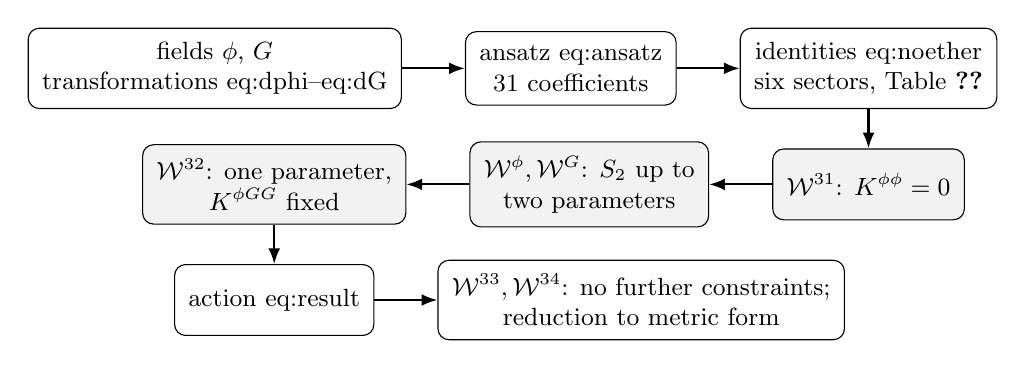
\begin{tikzpicture}[
  node distance=5mm and 8mm,
  box/.style={draw, rounded corners, align=center, minimum height=9mm, inner sep=5pt, font=\small},
  res/.style={box, fill=black!5},
  arr/.style={-{Latex[length=2mm]}, thick}]
\node[box] (fields) {fields $\phi$, $G$\\transformations \eqref{eq:dphi}--\eqref{eq:dG}};
\node[box, right=of fields] (ansatz) {ansatz \eqref{eq:ansatz}\\31 coefficients};
\node[box, right=of ansatz] (ident) {identities \eqref{eq:noether}\\six sectors, Table~\ref{tab:identities}};
\node[res, below=of ident] (khh) {$\W^{31}$: $K^{\phi\phi}=0$};
\node[res, left=of khh] (s2) {$\W^{\phi},\W^{G}$: $S_2$ up to\\two parameters};
\node[res, left=of s2] (s3) {$\W^{32}$: one parameter,\\$K^{\phi GG}$ fixed};
\node[box, below=of s3] (result) {action \eqref{eq:result}};
\node[box, right=of result] (check) {$\W^{33},\W^{34}$: no further constraints;\\reduction to metric form};
\draw[arr] (fields) -- (ansatz);
\draw[arr] (ansatz) -- (ident);
\draw[arr] (ident) -- (khh);
\draw[arr] (khh) -- (s2);
\draw[arr] (s2) -- (s3);
\draw[arr] (s3) -- (result);
\draw[arr] (result) -- (check);
\end{tikzpicture}
\caption{The determination of the action. Inputs on the top row; the sequential solution of
Table~\ref{tab:flow} on the middle row; output and checks on the bottom row.}
\label{fig:flow}
\end{figure}

% =======================================================================
\section{Conclusions}
\label{sec:conclusions}
% =======================================================================

The procedure described here identifies the Goldberg--Palatini action through the
Noether identities of its prescribed field transformations. Within the local,
Lorentz-covariant, parity-even ansatz with the prescribed derivative orders and the cubic
sector restricted to $\phi GG$, the 31 coefficients of the kernel bases (for $d\geq4$) are
reduced to a single overall constant.
In particular, the identities eliminate the quadratic $\phi\phi$ kernel and fix the relative
coefficients of the mixed $\phi G$ term, the algebraic $GG$ term, and the cubic $\phi GG$
interaction. The resulting structure is that of first-order Einstein gravity.

Individual Noether identities can leave components of a kernel undetermined, since they
constrain tensor contractions. Uniqueness here follows from imposing all identities
simultaneously within the chosen ansatz: the field-dependent transformations link the
quadratic and cubic sectors and remove the freedom left by the quadratic identities alone.
The resulting homogeneous linear system has a one-dimensional solution space, corresponding
to the overall normalization of the action. Any further independent solution would define
another invariant action in the same class. Thus uniqueness is a property of this restricted
system, not a general consequence of Noether identities. The connection is not a field
exempt from the procedure: its variation enters every sector of the identity except the
$\phi\phi$ one, and the coupled identities determine the kernels involving it; once the
preceding constraints are imposed, the cubic vertex is fixed by the sector that couples the
two fields, $\W^{32}$. The solution was obtained with the
momenta of the cubic identities identified; its invariance for arbitrary momenta follows
from its identification with the Goldberg--Palatini action.

For $d>2$ and nondegenerate metric density the algebraic equation for $G$ has a unique
solution, so fixing the first-order action fixes the second-order one completely.
Eliminating $G$ yields the metric action as the quadratic form \eqref{eq:second}, modulo a
boundary term and with the overall normalization inherited from the first-order action, and
the formal expansion of its kernel in powers of $\kappa$ produces every graviton
self-interaction vertex of the second-order theory. A construction that closes at cubic
order in the first-order variables therefore determines an infinite set of vertices in the
metric variables; this is the practical content of the classical equivalence between the two
formulations, and it is what makes the first-order variables the natural setting for the
determination.

The method makes the role of symmetry explicit at each order in the fields. It avoids
selecting an energy--momentum tensor as the source of successive self-couplings and instead
imposes off-shell relations directly on the action kernels. Its practical advantage is that
the polynomial first-order formulation turns the determination of the action into a finite tensor-algebra
problem.

A natural extension is to enlarge the interaction ansatz while retaining explicit control
over locality and derivative order. Terms involving additional powers of $\phi$, or
derivatives compatible with other cubic field combinations, would test whether the
restriction to $\phi GG$ can be relaxed without introducing new invariant structures.
For Yang--Mills theory the tree-amplitude version of the argument is known to close and
to fix the interaction structure under its stated assumptions~\cite{BrandtFrenkel1996}; the
action-level version with tensor bases would provide a direct check of the method, while higher-derivative gravitational
actions would allow it to probe a broader space of gauge-invariant dynamics.

\begin{acknowledgments}
\todo{Funding: CNPq grant of F.T.B.; PUB/USP scholarship of A.C.B.C.}
In preparing this manuscript the authors used AI language models (Claude, Anthropic, and
Codex, OpenAI) as editing and programming assistants: for revising the English text, for
organizing the appendices, and for writing and debugging parts of the symbolic-computation
notebooks and scripts. All physics content, derivations and checks were carried out and
verified by the authors, who take full responsibility for the paper.
\end{acknowledgments}

% =======================================================================
\appendix
% =======================================================================

\section{Derivation of the transformation laws}
\label{app:transf}

This appendix derives Eqs.~\eqref{eq:dphi} and \eqref{eq:dG} from the transformation
properties of $g_{\mu\nu}$ and $\Gamma^{\lambda}{}_{\mu\nu}$ under coordinate changes. They are Eqs.~(17b) and (18) of
Ref.~\cite{BrandtMcKeon2015}, whose Eq.~(17a) is the transformation of $h^{\mu\nu}$ itself,
Eq.~\eqref{eq:dh} below; the parameter $\theta$ of that reference is $-\kappa\omega$ here, and
that reference sets $\kappa=1$.

\paragraph{Conventions.} Under the infinitesimal coordinate change
$x'^\mu=x^\mu-\varepsilon^\mu(x)$ we define the variation of a field as
$\delta T(x)\equiv T'(x)-T(x)$. For a tensor this is the Lie derivative along $\varepsilon$,
$\delta T=\mathcal{L}_\varepsilon T$; for the objects needed below,
\begin{align}
\mathcal{L}_\varepsilon V^\mu&=\varepsilon^\rho\partial_\rho V^\mu-V^\rho\partial_\rho\varepsilon^\mu,\qquad
\mathcal{L}_\varepsilon T_\nu=\varepsilon^\rho\partial_\rho T_\nu+T_\rho\partial_\nu\varepsilon^\rho,\\
\mathcal{L}_\varepsilon X^{\lambda}{}_{\mu\nu}&=\varepsilon^\rho\partial_\rho X^{\lambda}{}_{\mu\nu}
-X^{\rho}{}_{\mu\nu}\partial_\rho\varepsilon^\lambda
+X^{\lambda}{}_{\rho\nu}\partial_\mu\varepsilon^\rho
+X^{\lambda}{}_{\mu\rho}\partial_\nu\varepsilon^\rho.
\label{eq:lie12}
\end{align}
$\mathcal{L}_\varepsilon$ is linear and obeys the Leibniz rule, and it annihilates the
Kronecker delta: $\mathcal{L}_\varepsilon\delta^\lambda_\mu
=-\delta^{\rho}_{\mu}\partial_\rho\varepsilon^\lambda+\delta^{\lambda}_{\rho}\partial_\mu\varepsilon^\rho=0$.
At the end we set $\varepsilon=\kappa\omega$, which is the parametrization of
Section~\ref{sec:variables}.

\paragraph{The metric density.} From $\delta g_{\mu\nu}=\mathcal{L}_\varepsilon g_{\mu\nu}$
and $\delta g^{\mu\nu}=-g^{\mu\alpha}g^{\nu\beta}\delta g_{\alpha\beta}$ one has
$\delta g^{\mu\nu}=\varepsilon^\rho\partial_\rho g^{\mu\nu}-g^{\rho\nu}\partial_\rho\varepsilon^\mu
-g^{\mu\rho}\partial_\rho\varepsilon^\nu$, and from
$\delta\sqrt{-g}=\tfrac12\sqrt{-g}\,g^{\alpha\beta}\delta g_{\alpha\beta}$ together with
$\partial_\rho\sqrt{-g}=\tfrac12\sqrt{-g}\,g^{\alpha\beta}\partial_\rho g_{\alpha\beta}$,
$\delta\sqrt{-g}=\varepsilon^\rho\partial_\rho\sqrt{-g}+\sqrt{-g}\,\partial_\rho\varepsilon^\rho$.
The product rule then gives, for $h^{\mu\nu}\equiv\sqrt{-g}\,g^{\mu\nu}$,
\begin{equation}
\delta h^{\mu\nu}=\partial_\rho\big(h^{\mu\nu}\varepsilon^\rho\big)
-h^{\rho\nu}\partial_\rho\varepsilon^\mu-h^{\mu\rho}\partial_\rho\varepsilon^\nu ,
\label{eq:dh}
\end{equation}
the transformation of a contravariant tensor density of weight one. Holding the background
$\eta^{\mu\nu}$ fixed, so that $\delta h^{\mu\nu}=\kappa\,\delta\phi^{\mu\nu}$, we insert
$h^{\mu\nu}=\eta^{\mu\nu}+\kappa\phi^{\mu\nu}$ and $\varepsilon=\kappa\omega$ and divide by
$\kappa$,
\begin{equation}
\delta\phi^{\mu\nu}=\eta^{\mu\nu}\partial\!\cdot\!\omega-\partial^{(\mu}\omega^{\nu)}
+\kappa\Big[\partial_\rho\big(\phi^{\mu\nu}\omega^\rho\big)-\partial_\rho\omega^{(\mu}\phi^{\nu)\rho}\Big],
\end{equation}
which is Eq.~\eqref{eq:dphi}.

\paragraph{The connection.} An affine connection transforms so that $\nabla_\mu V^\nu$ is a
tensor for every $V$; the infinitesimal form of the resulting law is the Lie derivative of a
$(1,2)$ tensor plus an inhomogeneous term,
\begin{equation}
\delta\Gamma^{\lambda}{}_{\mu\nu}=\mathcal{L}_\varepsilon\Gamma^{\lambda}{}_{\mu\nu}
+\partial_\mu\partial_\nu\varepsilon^\lambda .
\label{eq:dGamma}
\end{equation}
Here and below, when applied to the connection, to its trace or to the trace-adjusted
connection, $\mathcal{L}_\varepsilon$ denotes only the corresponding tensor-form expression;
the inhomogeneous terms, which make these objects non-tensorial, are displayed separately.

\paragraph{The trace.} Let $T_\nu\equiv\Gamma^{\lambda}{}_{\nu\lambda}$. Contracting
$\lambda$ with $\mu$ in Eq.~\eqref{eq:dGamma}, the second and third terms of the Lie derivative
\eqref{eq:lie12} become $-\Gamma^{\rho}{}_{\lambda\nu}\partial_\rho\varepsilon^\lambda
+\Gamma^{\lambda}{}_{\rho\nu}\partial_\lambda\varepsilon^\rho$ and cancel after renaming the
dummy indices, while the inhomogeneous term becomes $\partial_\nu(\partial\!\cdot\!\varepsilon)$:
\begin{equation}
\delta T_\nu=\mathcal{L}_\varepsilon T_\nu+\partial_\nu(\partial\!\cdot\!\varepsilon).
\label{eq:dT}
\end{equation}

\paragraph{The trace-adjusted connection.} By Eq.~\eqref{eq:Gdef},
$\Gamma^{\lambda}{}_{\mu\nu}=\kappa G^{\lambda}{}_{\mu\nu}
+\tfrac12\big(\delta^\lambda_\mu T_\nu+\delta^\lambda_\nu T_\mu\big)$, and therefore
$\delta(\kappa G)=\delta\Gamma-\tfrac12\big(\delta^\lambda_\mu\,\delta T_\nu+\delta^\lambda_\nu\,\delta T_\mu\big)$.
In $\delta\Gamma$, Eq.~\eqref{eq:dGamma}, the Lie derivative acts linearly on the two pieces of
$\Gamma$, and since it annihilates $\delta^\lambda_\mu$,
$\mathcal{L}_\varepsilon\big(\delta^\lambda_\mu T_\nu\big)=\delta^\lambda_\mu\,\mathcal{L}_\varepsilon T_\nu$.
Using Eq.~\eqref{eq:dT} for $\delta T$, the terms $\tfrac12\delta^\lambda_\mu\mathcal{L}_\varepsilon T_\nu
+\tfrac12\delta^\lambda_\nu\mathcal{L}_\varepsilon T_\mu$ cancel between $\delta\Gamma$ and
the trace correction, and what survives of the latter is the inhomogeneous part of
Eq.~\eqref{eq:dT}:
\begin{equation}
\delta(\kappa G^{\lambda}{}_{\mu\nu})=\kappa\,\mathcal{L}_\varepsilon G^{\lambda}{}_{\mu\nu}
+\partial_\mu\partial_\nu\varepsilon^\lambda
-\tfrac12\big(\delta^\lambda_\mu\partial_\nu+\delta^\lambda_\nu\partial_\mu\big)\partial\!\cdot\!\varepsilon .
\end{equation}
With $\varepsilon=\kappa\omega$ and Eq.~\eqref{eq:lie12} for $\mathcal{L}_\omega G$, this is
Eq.~\eqref{eq:dG}. The trace adjustment thus leaves the two-derivative term
$\partial_\mu\partial_\nu\omega^\lambda$ unchanged and subtracts
$\tfrac12(\delta^\lambda_\mu\partial_\nu+\delta^\lambda_\nu\partial_\mu)\partial\!\cdot\!\omega$,
so that the trace of the variation is
$\delta^{(0)}G^{\lambda}{}_{\nu\lambda}=\tfrac{1-d}{2}\,\partial_\nu\partial\!\cdot\!\omega$,
consistent with $\Gamma^{\sigma}{}_{\nu\sigma}=\frac{2\kappa}{1-d}g_\nu$; this is why
$\delta^{(0)}G$ is not simpler than $\delta^{(0)}\Gamma$ even though the action in the
variable $G$ is. Both Eq.~\eqref{eq:dT} and the final result were verified symbolically
(Appendix~\ref{app:implementation}).

\section{Transformations in momentum space}
\label{app:momentum}

With the Fourier conventions of Section~\ref{sec:variables}, Eq.~\eqref{eq:dmom} reads, with
all indices displayed,
\begin{align}
\delta\p^{\mu\nu}(p)&=D_{\phi^0}{}^{\mu\nu}{}_{\alpha}(p)\,\tomega^\alpha(p)
+\kappa\ip{q}\p^{\alpha\beta}(p-q)\,\tomega^\rho(q)\,D_{\phi^1}{}^{\mu\nu}{}_{\alpha\beta\rho}(p,q),\\
\delta\G^{\lambda}{}_{\mu\nu}(p)&=D_{G^0}{}^{\lambda}{}_{\mu\nu\alpha}(p)\,\tomega^\alpha(p)
+\kappa\ip{q}\G^{\alpha}{}_{\beta\gamma}(p-q)\,\tomega^\rho(q)\,
D_{G^1}{}^{\lambda}{}_{\mu\nu\alpha}{}^{\beta\gamma}{}_{\rho}(p,q),
\end{align}
with
\begin{align}
D_{\phi^0}{}^{\mu\nu}{}_{\alpha}(p)&=-i\big(\eta^{\mu\nu}p_\alpha-p^{(\mu}\delta^{\nu)}_{\alpha}\big),\\
D_{\phi^1}{}^{\mu\nu}{}_{\alpha\beta\rho}(p,q)&=-i\big(\delta^{\mu}_{\alpha}\delta^{\nu}_{\beta}\,p_\rho
-q_\beta\,\delta^{(\mu}_{\alpha}\delta^{\nu)}_{\rho}\big),\\
D_{G^0}{}^{\lambda}{}_{\mu\nu\alpha}(p)&=-p_\mu p_\nu\delta^{\lambda}_{\alpha}
+\tfrac12\delta^{\lambda}_{(\mu}p_{\nu)}p_\alpha,\\
D_{G^1}{}^{\lambda}{}_{\mu\nu\alpha}{}^{\beta\gamma}{}_{\rho}(p,q)&=-i\big[
\delta^{\lambda}_{\alpha}\delta^{\beta}_{\mu}\delta^{\gamma}_{\nu}\,(p-q)_\rho
-q_\alpha\,\delta^{\beta}_{\mu}\delta^{\gamma}_{\nu}\delta^{\lambda}_{\rho}
+\delta^{\lambda}_{\alpha}\delta^{\beta}_{\rho}\delta^{\gamma}_{(\mu}q_{\nu)}\big].
\end{align}
These expressions are understood as maps acting on fields with their stated index
symmetries; symmetrization in the contracted field slots is therefore implicit, and a
representative differing by terms that vanish on symmetric fields defines the same map.

\section{Tensor bases}
\label{app:bases}

Each kernel is expanded in the basis of all independent tensors with its index structure,
built from $\eta$ and $p$ with the momentum dependence of Table~\ref{tab:kernels}. The
construction is the same for the four kernels. One enumerates the tensor monomials of the
required degree in $p$, each a single product of $\eta$'s over the index slots (index
positions of $K$) not carrying a
momentum, times the appropriate powers of $p$, and symmetrizes each monomial under the
index symmetries of the kernel. These symmetries, listed in Table~\ref{tab:kernels}, generate
a finite group $\mathsf{G}_K$ of permutations of the index slots of $K$. Applying every
element of $\mathsf{G}_K$ to a monomial $T$ produces a set of $n$ distinct monomials
$T_1,\dots,T_n$, the \emph{orbit} of $T$; the symmetrized monomial is the average over the
orbit, $\mathcal{S}[T]=\frac1n\sum_{k=1}^{n}T_k$ (equivalently, the average of $T$ over the
group). Two monomials give the same $\mathcal{S}[T]$ if and only if they lie in the same
orbit, so the orbit averages form a basis of the invariant formal expressions, in
one-to-one correspondence with the orbits, and any element of an orbit may serve as its
representative. This is a candidate tensor basis; its independence as a set of tensors in a
given dimension is checked below. The orbit sizes $n$ add up to the number of monomials.

Tables~\ref{tab:basis-phiphi}--\ref{tab:basis-phiGG} list, for each kernel, a representative
monomial of every orbit and the number $n$ of terms in the corresponding symmetrized sum.
Indices are written in the order of the kernel's slots; $p^2\equiv p_\alpha p^\alpha$. For
$K^{\phi\phi}$, for instance, element~4 of Table~\ref{tab:basis-phiphi} is
$\tfrac14\big(p_\mu p_\rho\eta_{\nu\sigma}+p_\nu p_\rho\eta_{\mu\sigma}
+p_\mu p_\sigma\eta_{\nu\rho}+p_\nu p_\sigma\eta_{\mu\rho}\big)$.

Distinct orbits have disjoint monomial content, so the elements are linearly independent as
formal expressions. They can nevertheless become dependent as tensors in low dimension,
through identities that hold only for specific $d$. Independence for generic $d$ is verified by
computing the Gram matrix $\Gamma_K$ of each basis, $(\Gamma_K)_{ij}=\mathcal{S}[T_i]\cdot\mathcal{S}[T_j]$
with all indices contracted, and checking that its determinant is not identically zero; the
determinant is a polynomial in $d$ whose zeros locate the dimensions where the basis
degenerates. A nonzero determinant establishes linear independence in any signature. Since
the entries of $\Gamma_K$ depend on the signature only through $d$ and $p^2$, the
dimension-dependent degeneracies can be identified at nonzero Euclidean momentum, where the
contraction pairing is positive definite and a vanishing determinant does imply linear
dependence; the resulting polynomial tensor relations hold in Lorentzian signature as well. For the bases of Tables~\ref{tab:basis-phiphi}--\ref{tab:basis-phiGG}, up to
positive numerical factors,
\begin{align}
\det\Gamma_{\phi\phi}&=(p^2)^8\,(d-2)(d-1)^3(d+2)(d+4),\\
\det\Gamma_{\phi G}&=(p^2)^6\,(d-2)(d-1)^5(d+2)^5(d+4),\\
\det\Gamma_{GG}&=d^5\,(d-2)(d-1)^4(d+2)^4(d+4),\\
\det\Gamma_{\phi GG}&=d^{16}\,(d-3)(d-2)^7(d-1)^{15}(d+1)^3(d+2)^{15}(d+4)^6(d+6).
\end{align}
All four are nonzero for $d\geq4$ and $p^2\neq0$; the powers of $p^2$ reflect the momentum
dependence of the first two bases and are unrelated to dimension-dependent relations. The
zeros at $d=1,2$, and at $d=3$ for $K^{\phi GG}$,
are the low dimensions in which products of $\eta$'s with many indices become linearly
dependent (in $d=3$, for instance, antisymmetrization over four indices vanishes).

\begin{table}[htb]
\centering
\begin{tabular}{@{}cl c@{}}
\toprule
& Representative monomial & $n$ \\
\midrule
1 & $p^2\,\eta_{\mu\nu}\eta_{\rho\sigma}$ & 1 \\
2 & $p^2\,\eta_{\mu\rho}\eta_{\nu\sigma}$ & 2 \\
3 & $p_{\mu}p_{\nu}\eta_{\rho\sigma}$ & 2 \\
4 & $p_{\mu}p_{\rho}\eta_{\nu\sigma}$ & 4 \\
\bottomrule
\end{tabular}
\caption{Basis of $K^{\phi\phi}_{\mu\nu\rho\sigma}(p)$: 4 elements, the orbits of the 9 monomials
under the symmetry group of order 8.}
\label{tab:basis-phiphi}
\end{table}

\begin{table}[htb]
\centering
\begin{tabular}{@{}cl c@{}}
\toprule
& Representative monomial & $n$ \\
\midrule
1 & $p_{\mu}\eta_{\nu\lambda}\eta_{\rho\sigma}$ & 2 \\
2 & $p_{\mu}\eta_{\nu\rho}\eta_{\lambda\sigma}$ & 4 \\
3 & $p_{\lambda}\eta_{\mu\nu}\eta_{\rho\sigma}$ & 1 \\
4 & $p_{\lambda}\eta_{\mu\rho}\eta_{\nu\sigma}$ & 2 \\
5 & $p_{\rho}\eta_{\mu\nu}\eta_{\lambda\sigma}$ & 2 \\
6 & $p_{\rho}\eta_{\mu\lambda}\eta_{\nu\sigma}$ & 4 \\
\bottomrule
\end{tabular}
\caption{Basis of $K^{\phi G}_{\mu\nu\lambda\rho\sigma}(p)$: 6 elements, the orbits of the 15
monomials under the symmetry group of order 4.}
\label{tab:basis-phiG}
\end{table}

\begin{table}[htb]
\centering
\begin{tabular}{@{}cl c@{}}
\toprule
& Representative monomial & $n$ \\
\midrule
1 & $\eta_{\lambda\mu}\eta_{\nu\rho}\eta_{\sigma\tau}$ & 4 \\
2 & $\eta_{\lambda\mu}\eta_{\nu\sigma}\eta_{\rho\tau}$ & 4 \\
3 & $\eta_{\lambda\rho}\eta_{\mu\nu}\eta_{\sigma\tau}$ & 1 \\
4 & $\eta_{\lambda\rho}\eta_{\mu\sigma}\eta_{\nu\tau}$ & 2 \\
5 & $\eta_{\lambda\sigma}\eta_{\mu\rho}\eta_{\nu\tau}$ & 4 \\
\bottomrule
\end{tabular}
\caption{Basis of $K^{GG}_{\lambda\mu\nu\rho\sigma\tau}$: 5 elements, the orbits of the 15
monomials under the symmetry group of order 8.}
\label{tab:basis-GG}
\end{table}

\begin{table}[htb]
\centering
\setlength{\aboverulesep}{0pt}\setlength{\belowrulesep}{0pt}\renewcommand{\arraystretch}{1.15}
\begin{tabular}{@{}cl c@{\hspace{5pt}}|@{\hspace{5pt}}cl c@{}}
\toprule
& Representative monomial & $n$ & & Representative monomial & $n$ \\
\midrule
1 & $\eta_{\mu\nu}\eta_{\lambda\alpha}\eta_{\beta\rho}\eta_{\sigma\tau}$ & 4 & 9 & $\eta_{\mu\lambda}\eta_{\nu\rho}\eta_{\alpha\sigma}\eta_{\beta\tau}$ & 4 \\
2 & $\eta_{\mu\nu}\eta_{\lambda\alpha}\eta_{\beta\sigma}\eta_{\rho\tau}$ & 4 & 10 & $\eta_{\mu\lambda}\eta_{\nu\sigma}\eta_{\alpha\beta}\eta_{\rho\tau}$ & 8 \\
3 & $\eta_{\mu\nu}\eta_{\lambda\rho}\eta_{\alpha\beta}\eta_{\sigma\tau}$ & 1 & 11 & $\eta_{\mu\lambda}\eta_{\nu\sigma}\eta_{\alpha\rho}\eta_{\beta\tau}$ & 16 \\
4 & $\eta_{\mu\nu}\eta_{\lambda\rho}\eta_{\alpha\sigma}\eta_{\beta\tau}$ & 2 & 12 & $\eta_{\mu\alpha}\eta_{\nu\beta}\eta_{\lambda\rho}\eta_{\sigma\tau}$ & 4 \\
5 & $\eta_{\mu\nu}\eta_{\lambda\sigma}\eta_{\alpha\rho}\eta_{\beta\tau}$ & 4 & 13 & $\eta_{\mu\alpha}\eta_{\nu\beta}\eta_{\lambda\sigma}\eta_{\rho\tau}$ & 8 \\
6 & $\eta_{\mu\lambda}\eta_{\nu\alpha}\eta_{\beta\rho}\eta_{\sigma\tau}$ & 8 & 14 & $\eta_{\mu\alpha}\eta_{\nu\sigma}\eta_{\lambda\beta}\eta_{\rho\tau}$ & 8 \\
7 & $\eta_{\mu\lambda}\eta_{\nu\alpha}\eta_{\beta\sigma}\eta_{\rho\tau}$ & 16 & 15 & $\eta_{\mu\alpha}\eta_{\nu\sigma}\eta_{\lambda\rho}\eta_{\beta\tau}$ & 8 \\
8 & $\eta_{\mu\lambda}\eta_{\nu\rho}\eta_{\alpha\beta}\eta_{\sigma\tau}$ & 2 & 16 & $\eta_{\mu\alpha}\eta_{\nu\sigma}\eta_{\lambda\tau}\eta_{\beta\rho}$ & 8 \\
\bottomrule
\end{tabular}
\caption{Basis of $K^{\phi GG}_{\mu\nu\lambda\alpha\beta\rho\sigma\tau}$: 16 elements, the
orbits of the 105 monomials (one for each perfect matching of the eight index slots by four
$\eta$'s) under the symmetry group of order 16.}
\label{tab:basis-phiGG}
\end{table}

\section{The six identities}
\label{app:identities}

In the notation of Section~\ref{sec:variables}, each identity of Table~\ref{tab:identities}
states that a multilinear form in the fields and the gauge parameter vanishes identically.
Writing $P$ for the total momentum ($P=p_1+p_2$ or $p_1+p_2+p_3$), the six forms are
\begin{align}
\W^{\phi}:&\quad 2K^{\phi\phi}\big(\phi_{-p},D_{\phi^0}(p)\,\omega_p\big)
+K^{\phi G}\big(\phi_{-p},D_{G^0}(p)\,\omega_p\big)=0,\\
\W^{G}:&\quad K^{\phi G}\big(D_{\phi^0}(p)\,\omega_p,G_{-p}\big)
+2K^{GG}\big(G_{-p},D_{G^0}(p)\,\omega_p\big)=0,\\
\W^{31}:&\quad K^{\phi\phi}\big(\phi_{-p_1},D_{\phi^1}(p_1,P)(\phi_{-p_2},\omega_P)\big)
+(1\leftrightarrow2)=0,\\
\begin{split}
\W^{32}:&\quad 2K^{\phi GG}\big(\phi_{-p_2},D_{G^0}(P)\,\omega_P,G_{-p_1}\big)
+K^{\phi G}\big(D_{\phi^1}(p_1,P)(\phi_{-p_2},\omega_P),G_{-p_1}\big)\\
&\quad+K^{\phi G}\big(\phi_{-p_2},D_{G^1}(p_2,P)(G_{-p_1},\omega_P)\big)=0,
\end{split}\\
\begin{split}
\W^{33}:&\quad K^{\phi GG}\big(D_{\phi^0}(P)\,\omega_P,G_{-p_1},G_{-p_2}\big)
+K^{GG}\big(G_{-p_1},D_{G^1}(p_1,P)(G_{-p_2},\omega_P)\big)+(1\leftrightarrow2)=0,
\end{split}\\
\begin{split}
\W^{34}:&\quad K^{\phi GG}\big(\phi_{-p_3},G_{-p_1},D_{G^1}(p_1+p_3,P)(G_{-p_2},\omega_P)\big)
+(1\leftrightarrow2)\\
&\quad+K^{\phi GG}\big(D_{\phi^1}(p_1+p_2,P)(\phi_{-p_3},\omega_P),G_{-p_1},G_{-p_2}\big)=0,
\end{split}
\end{align}
where $(1\leftrightarrow2)$ adds the immediately preceding term with the two field
arguments of the same type exchanged, that is, with $p_1\leftrightarrow p_2$ and, in the
component form below, with their index groups exchanged as well; in $\W^{33}$ it applies
only to the $K^{GG}$ term. The factors of two count the two equal contributions of a kernel
that is quadratic in the field being varied. Each term is one kernel of
Eq.~\eqref{eq:ansatz} with one argument replaced by the appropriate piece of the
transformation \eqref{eq:dmom}, the momenta being fixed by momentum conservation. Since the
fields are arbitrary within their symmetry classes, the coefficient tensor of
$\phi_{-p_1}\cdots\omega_P$ in each form, projected onto the index symmetries of the field
slots, vanishes. With all indices displayed, and in terms
of the tensors of Appendix~\ref{app:momentum}, these coefficient tensors are
\begin{align}
\W^{\phi}_{\rho\sigma\alpha}(p)&\equiv
2D_{\phi^0}{}^{\mu\nu}{}_{\alpha}(p)K^{\phi\phi}_{\mu\nu\rho\sigma}(p)
+D_{G^0}{}^{\lambda}{}_{\mu\nu\alpha}(p)K^{\phi G}_{\rho\sigma\lambda}{}^{\mu\nu}(p)=0,\\
\W^{G}_{\rho\sigma\tau\alpha}(p)&\equiv
D_{\phi^0}{}^{\mu\nu}{}_{\alpha}(p)K^{\phi G}_{\mu\nu\rho\sigma\tau}(-p)
+2D_{G^0}{}^{\lambda}{}_{\mu\nu\alpha}(p)K^{GG}_{\lambda}{}^{\mu\nu}{}_{\rho\sigma\tau}=0,\\
\begin{split}
\W^{31}_{\mu_1\nu_1\mu_2\nu_2\rho}(p_1,p_2)&\equiv
K^{\phi\phi}_{\mu_1\nu_1\alpha\beta}(p_1)D_{\phi^1}{}^{\alpha\beta}{}_{\mu_2\nu_2\rho}(p_1,p_1+p_2)\\
&\quad+K^{\phi\phi}_{\mu_2\nu_2\alpha\beta}(p_2)D_{\phi^1}{}^{\alpha\beta}{}_{\mu_1\nu_1\rho}(p_2,p_1+p_2)=0,
\end{split}\\
\begin{split}
\W^{32}_{\lambda_1\mu_1\nu_1\mu_2\nu_2\rho}(p_1,p_2)&\equiv
2K^{\phi GG}_{\mu_2\nu_2\lambda\mu\nu\lambda_1\mu_1\nu_1}D_{G^0}{}^{\lambda\mu\nu}{}_{\rho}(p_1+p_2)\\
&\quad+K^{\phi G}_{\mu\nu\lambda_1\mu_1\nu_1}(-p_1)D_{\phi^1}{}^{\mu\nu}{}_{\mu_2\nu_2\rho}(p_1,p_1+p_2)\\
&\quad+K^{\phi G}_{\mu_2\nu_2\lambda}{}^{\mu\nu}(p_2)D_{G^1}{}^{\lambda}{}_{\mu\nu\lambda_1\mu_1\nu_1\rho}(p_2,p_1+p_2)=0,
\end{split}\\
\begin{split}
\W^{33}_{\lambda_1\mu_1\nu_1\lambda_2\mu_2\nu_2\rho}(p_1,p_2)&\equiv
K^{\phi GG}_{\mu\nu\lambda_1\mu_1\nu_1\lambda_2\mu_2\nu_2}D_{\phi^0}{}^{\mu\nu}{}_{\rho}(p_1+p_2)\\
&\quad+K^{GG}_{\lambda\mu\nu\lambda_1\mu_1\nu_1}D_{G^1}{}^{\lambda\mu\nu}{}_{\lambda_2\mu_2\nu_2\rho}(p_1,p_1+p_2)\\
&\quad+K^{GG}_{\lambda\mu\nu\lambda_2\mu_2\nu_2}D_{G^1}{}^{\lambda\mu\nu}{}_{\lambda_1\mu_1\nu_1\rho}(p_2,p_1+p_2)=0,
\end{split}\\
\begin{split}
\W^{34}_{\lambda_1\mu_1\nu_1\lambda_2\mu_2\nu_2\mu_3\nu_3\rho}(p_1,p_2,p_3)&\equiv\\
&\quad\phantom{+}K^{\phi GG}_{\mu_3\nu_3\lambda\mu\nu\lambda_1\mu_1\nu_1}D_{G^1}{}^{\lambda\mu\nu}{}_{\lambda_2\mu_2\nu_2\rho}(p_1+p_3,P)\\
&\quad+K^{\phi GG}_{\mu_3\nu_3\lambda\mu\nu\lambda_2\mu_2\nu_2}D_{G^1}{}^{\lambda\mu\nu}{}_{\lambda_1\mu_1\nu_1\rho}(p_2+p_3,P)\\
&\quad+K^{\phi GG}_{\mu\nu\lambda_1\mu_1\nu_1\lambda_2\mu_2\nu_2}D_{\phi^1}{}^{\mu\nu}{}_{\mu_3\nu_3\rho}(p_1+p_2,P)=0,
\end{split}
\end{align}
The identities above retain their generic momentum dependence. For the projection bases
of the cubic identities the independent momenta are identified, $p_1=p_2=p$, and also
$p_3=p$ in $\W^{34}$, as explained in Section~\ref{sec:identities}. The projection bases of
Table~\ref{tab:identities} are generated by the procedure of Appendix~\ref{app:bases}, from
the monomials with the index structure and degree in $p$ of each identity, averaged over its
symmetry group: the symmetries of the kernel slots involved
and, for $\W^{31}$, $\W^{33}$ and $\W^{34}$, the exchange of the two identical fields.
Table~\ref{tab:proj} lists the three smallest ones as an illustration; the remaining
dimensions, 23, 20 and 95, make an explicit listing unhelpful, and those bases are generated
by the code of Appendix~\ref{app:implementation}. Their Gram determinants are, up to
numerical factors, $(p^2)^9(d-1)^2$, $(p^2)^{12}(d-2)(d-1)^5(d+2)(d+4)$ and
$(p^2)^{21}(d-2)^2(d-1)^6(d+1)(d+4)(d+6)$ for the three bases of Table~\ref{tab:proj}, and
for $p^2\neq0$ those of the bases of $\W^{32}$ and $\W^{33}$ vanish, among positive
integer dimensions, only at $d=1,2,3$; all five are therefore nondegenerate for $d\geq4$ and
$p^2\neq0$. The basis of $\W^{34}$ becomes degenerate at $d=4$. This does not obstruct the
determination, since no inversion of that Gram matrix is needed: the other identities fix
the kernels, $\W^{34}$ is then found to be satisfied identically by substitution, and its
vanishing also follows from the identification of the solution with the invariant
Goldberg--Palatini action.

\begin{table}[htb]
\centering\footnotesize
\setlength{\aboverulesep}{0pt}\setlength{\belowrulesep}{0pt}\renewcommand{\arraystretch}{1.15}
\begin{tabular}{@{}cl c@{\hspace{5pt}}|@{\hspace{5pt}}cl c@{}}
\toprule
& Representative monomial & $n$ & & Representative monomial & $n$ \\
\midrule
\multicolumn{3}{@{}l@{\hspace{5pt}}|@{\hspace{5pt}}}{$\W^{\phi}_{\rho\sigma\alpha}(p)$} & \multicolumn{3}{l@{}}{$\W^{31}_{\mu_1\nu_1\mu_2\nu_2\rho}(p,p)$} \\
1 & $p_{\rho}p_{\sigma}p_{\alpha}$ & 1 & 1 & $p_{\mu_1}p_{\nu_1}p_{\rho}\eta_{\mu_2\nu_2}$ & 2 \\
2 & $p^2\,p_{\alpha}\eta_{\rho\sigma}$ & 1 & 2 & $p_{\mu_1}p_{\nu_1}p_{\mu_2}\eta_{\nu_2\rho}$ & 4 \\
3 & $p^2\,p_{\rho}\eta_{\sigma\alpha}$ & 2 & 3 & $p_{\mu_1}p_{\mu_2}p_{\rho}\eta_{\nu_1\nu_2}$ & 4 \\
\multicolumn{3}{@{}l@{\hspace{5pt}}|@{\hspace{5pt}}}{$\W^{G}_{\rho\sigma\tau\alpha}(p)$} & 4 & $p^2\,p_{\rho}\eta_{\mu_1\nu_1}\eta_{\mu_2\nu_2}$ & 1 \\
1 & $p_{\rho}p_{\alpha}\eta_{\sigma\tau}$ & 1 & 5 & $p^2\,p_{\rho}\eta_{\mu_1\mu_2}\eta_{\nu_1\nu_2}$ & 2 \\
2 & $p_{\sigma}p_{\tau}\eta_{\rho\alpha}$ & 1 & 6 & $p^2\,p_{\mu_1}\eta_{\nu_1\rho}\eta_{\mu_2\nu_2}$ & 4 \\
3 & $p_{\rho}p_{\sigma}\eta_{\tau\alpha}$ & 2 & 7 & $p^2\,p_{\mu_1}\eta_{\nu_1\mu_2}\eta_{\nu_2\rho}$ & 8 \\
4 & $p_{\sigma}p_{\alpha}\eta_{\rho\tau}$ & 2 & \multicolumn{3}{l@{}}{} \\
5 & $p^2\,\eta_{\rho\alpha}\eta_{\sigma\tau}$ & 1 & \multicolumn{3}{l@{}}{} \\
6 & $p^2\,\eta_{\rho\sigma}\eta_{\tau\alpha}$ & 2 & \multicolumn{3}{l@{}}{} \\
\bottomrule
\end{tabular}
\caption{The three smallest projection bases, in the notation of Appendix~\ref{app:bases}:
3, 6 and 7 elements, the orbits of 4, 9 and 25 monomials under symmetry groups of order 2, 2
and 8. For $\W^{31}$ the two momenta are identified, $p_1=p_2=p$, and the symmetry group
includes the exchange $(\mu_1\nu_1)\leftrightarrow(\mu_2\nu_2)$.}
\label{tab:proj}
\end{table}

\section{Explicit kernels}
\label{app:kernels}

Up to the overall constant, the solution of Table~\ref{tab:flow} is, in terms of the basis
elements $\mathcal{S}[T]$ of Appendix~\ref{app:bases} (the average of the monomial $T$ over
its orbit), and with all indices of the kernels lowered, to be raised with $\eta^{\mu\nu}$
as required by the contractions with the fields,
\begin{align}
K^{\phi\phi}_{\mu\nu\rho\sigma}(p)&=0,\\
K^{\phi G}_{\mu\nu\lambda\rho\sigma}(p)&=-i\,\mathcal{S}\big[p_\lambda\eta_{\mu\rho}\eta_{\nu\sigma}\big]
=-\tfrac{i}{2}\,p_\lambda\big(\eta_{\mu\rho}\eta_{\nu\sigma}+\eta_{\mu\sigma}\eta_{\nu\rho}\big),\\
\begin{split}
K^{GG}_{\lambda\mu\nu\rho\sigma\tau}&=
-\mathcal{S}\big[\eta_{\lambda\sigma}\eta_{\mu\rho}\eta_{\nu\tau}\big]
+\frac{1}{d-1}\,\mathcal{S}\big[\eta_{\lambda\mu}\eta_{\nu\sigma}\eta_{\rho\tau}\big]\\
&=\tfrac14\Big[-\eta_{\lambda(\sigma}\eta_{\tau)(\mu}\eta_{\nu)\rho}
+\frac{1}{d-1}\,\eta_{\lambda(\mu}\eta_{\nu)(\sigma}\eta_{\tau)\rho}\Big],
\end{split}\\
K^{\phi GG}_{\mu\nu\lambda\alpha\beta\rho\sigma\tau}&=
-\mathcal{S}\big[\eta_{\mu\alpha}\eta_{\nu\sigma}\eta_{\lambda\tau}\eta_{\beta\rho}\big]
+\frac{1}{d-1}\,\mathcal{S}\big[\eta_{\mu\alpha}\eta_{\nu\sigma}\eta_{\lambda\beta}\eta_{\rho\tau}\big],
\end{align}
that is, element~4 of Table~\ref{tab:basis-phiG}, elements 5 and 2 of
Table~\ref{tab:basis-GG}, and elements 16 and 14 of Table~\ref{tab:basis-phiGG}; the latter
two basis elements contain eight terms each. In the $GG$ and $\phi GG$ kernels the first
structure contracts the connection index of one $G$ with a lower index of the other, and the
second is the product of the two traces $g_\mu\equiv G^{\sigma}{}_{\mu\sigma}$.
Contracted with the fields, in the notation of Section~\ref{sec:variables}, these give
\begin{align}
K^{\phi G}(\phi_{-p},G_p)&=-ip_\lambda\,\p^{\mu\nu}(-p)\G^{\lambda}{}_{\mu\nu}(p),\\
K^{GG}(G_{-p},G_p)&=
\eta^{\mu\nu}\Big(-\G^{\lambda}{}_{\mu\sigma}(-p)\G^{\sigma}{}_{\nu\lambda}(p)+\frac{1}{d-1}\G^{\sigma}{}_{\mu\sigma}(-p)\G^{\rho}{}_{\nu\rho}(p)\Big),\\
K^{\phi GG}(\phi_{p+q},G_{-p},G_{-q})&=
\p^{\mu\nu}(p+q)\Big(-\G^{\lambda}{}_{\mu\sigma}(-p)\G^{\sigma}{}_{\nu\lambda}(-q)+\frac{1}{d-1}\G^{\sigma}{}_{\mu\sigma}(-p)\G^{\rho}{}_{\nu\rho}(-q)\Big),
\end{align}
whose inverse Fourier transform yields Eq.~\eqref{eq:result}, after an integration by parts
in the $\phi G$ term.

\section{Symbolic implementation and reproducibility}
\label{app:implementation}

In the first-order bootstrap implementation the coupling is set to $\kappa=1$. Since
$\kappa$ enters the construction only as the overall factor of $S_3$ in Eq.~\eqref{eq:ansatz}
and of $\delta^{(1)}$ in Eq.~\eqref{eq:dmom}, this affects neither the kernels of
Appendix~\ref{app:kernels} nor the identities of Appendix~\ref{app:identities}; it is restored
in the results by dimensional analysis, as in Section~\ref{sec:ansatz}. The second-order
comparison keeps $\kappa$ symbolic throughout.

\paragraph{Files.} The calculations are organized in the following Mathematica~\cite{Mathematica}
notebooks and data files, kept together in one directory.
\begin{enumerate}
\item \texttt{Goldberg\_Palatini\_Bootstrap\_en.nb} (FeynCalc~\cite{FeynCalc}): the first-order
determination. It generates the tensor bases of the four kernels and of the six identities
(Appendices~\ref{app:bases} and \ref{app:identities}) and the Gram determinants of the kernel
bases and of the five smallest projection bases (the rank test of the 95-element basis of
$\W^{34}$ at $d=4$ is an optional diagnostic, not part of the main flow), builds the
nonlinear identities with the field momenta identified, solves the linear system in the sequence of
Table~\ref{tab:flow}, checks the resulting kernels against Eqs.~(3.5)--(3.6) of
Ref.~\cite{BrandtMcKeon2016}, verifies the complete cubic kernel against $\tfrac12M(\phi)$
(cell tagged \texttt{FullCubicKernelCheck}), and exports the normalized kernels.
\item \texttt{Goldberg\_Palatini\_Bootstrap\_kernels.wl}: the exported kernels $K^{GG}$ and
$K^{\phi GG}$ in a package-independent slot representation, with the conventions
(dimension symbol, symmetries, normalization $c_{GG}=1/(d-1)$, Fourier sign); it is data,
not an executable script.
\item \texttt{Goldberg\_Palatini\_Cubic\_CLM.nb} (xAct/xTensor, xTras and xPerm~\cite{xPerm}):
the second-order comparison of Section~\ref{sec:checks}. It imports the data file without
FeynCalc, converts it to xAct tensors, derives $M_0^{-1}$ by solving its defining identity in
a five-element basis of metric structures and checks both inverse relations
(\texttt{inverseChecks}), substitutes $G_0$ back into $M_0G_0=\partial\phi$ as a test of index
placement and normalization (\texttt{g0Check}), and evaluates the residuals of
Eqs.~\eqref{eq:clm-quadratic}--\eqref{eq:clm-cubic}
(\texttt{clmQuadraticCheck}, \texttt{quadraticBoundaryCheck}, \texttt{clmCubicResidual});
\texttt{allChecksPassed} only aggregates these residuals. The notebook uses the
metric-compatible derivative of the flat background, \texttt{CD}, which in Cartesian
coordinates is the partial derivative of the text; the dimension is kept symbolic, and the
pole of $M_0^{-1}$ at $d=2$ is separate from the domain $d\geq4$ of the bases.
\end{enumerate}
A \texttt{README} gives the evaluation order (the first notebook and its export cell first;
the comparison notebook in a fresh kernel), the required packages and versions, the expected
result of every check, the conventions of the comparison, and the correspondence between the
notebooks and the equations and tables of this paper.

\todo{Procedure to make the code executable by anyone, to be completed before submission
(this note is to be removed from the final version, leaving only the files, requirements and
instructions actually available):
(i) assemble the public bundle with the files above, the README (already written) and the
drivers of item (ii), without backup copies or private paths (all input/output relative to the notebook or
script directory; the notebooks may keep their formatting and front-end output);
(ii) write one plain-text driver per notebook
(\texttt{.wls}) that runs under \texttt{wolframscript} without a front end, prints each
check and its residual, and exits with an error if any residual is nonzero;
(iii) install the Wolfram Engine on a clean machine under its free license, which requires
an account, activation and acceptance of its terms,
together with FeynCalc, xAct, xTras and xPerm, and run the drivers there; record the exact
versions and the outputs in the README; (iv) publish the bundle in a public repository
with a tagged release and a Zenodo DOI, and cite it here and in a data-availability
statement, not in the abstract; (v) only then state that the calculations can be
reproduced without a paid Mathematica license, for the uses permitted by the terms of the
free Wolfram Engine license. The Wolfram Engine is free but not license-free, and
notebooks need either the Mathematica front end or the drivers of item (ii). A route with no Wolfram license at all would require re-implementing
the checks in free software (the bases and Gram determinants already exist as Python/SymPy
scripts); whether to include such a re-implementation is left open.}

The notebooks and data files will be made available at \todo{repository URL and Zenodo DOI}.


\bibliographystyle{apsrev4-2}
\bibliography{bootstrap_refs}

\end{document}
